\documentclass[12pt]{article}
\usepackage{titlesec}
\usepackage{subcaption}
\usepackage[scaled]{helvet}  \renewcommand\familydefault{\sfdefault} % Font
\usepackage{graphicx} % Required for inserting images
\usepackage{geometry}
\usepackage{pgfplotstable}
\usepackage{amsmath}
\usepackage{enumitem}
\usepackage{tikz} 
\usetikzlibrary{petri,arrows.meta}
\geometry{a4paper, total={170mm,257mm},left=20mm, top=20mm,}
\usepackage[listings,breakable,skins]{tcolorbox}
% declare our code block environment
  \newtcblisting{tcbcodeblock}[1]{%
    enhanced,
    sharp corners,
    colframe=black,
    coltext=codefg,
    colback=codebg,
    breakable,
    size=fbox,
    listing only,
    listing options={%
      style=tcblatex,
      language={#1},
      showspaces=false,
      showstringspaces=false,
      commentstyle=\color{codegray},
      keywordstyle=\color{codegreen},
      stringstyle=\color{codecyan},
      basicstyle=\ttfamily\footnotesize
    }
  }
\renewcommand{\thesection}{\Roman{section}}
\renewcommand{\thesubsection}{\arabic{subsection}}
\renewcommand{\thesubsubsection}{\alph{subsubsection}.}

\titleformat{\section}{\normalfont\LARGE\bfseries}{\thesection.}{10pt}{}
\titleformat{\subsection}{\normalfont\Large}{\thesubsection.}{10pt}{}
\titleformat{\subsubsection}{\normalfont\large}{\thesubsubsection}{10pt}{}

\begin{document}
\thispagestyle{empty} %Suppress number of this page
\begin{center}
    \vspace{7pt}
    \fontsize{18pt}{17pt}\selectfont 
    \textbf{University of Science and Technology of Hanoi}
    \vspace{7pt}
\end{center}
\vspace{10pt}
\begin{center}
    
\includegraphics[scale=0.4]{images/USTH.png}
\end{center}

\vspace{90pt}

\begin{center}
    \fontsize{30pt}{17pt}\selectfont 
    \textbf{Deep Learning} 
    \vspace{50pt}

    \fontsize{20pt}{17pt}\selectfont 
    \textbf{Report 1 Gradient descend}
    \vspace{50pt}


    \fontsize{17pt}{17pt}\selectfont
    \textbf{{Student id: }{ict2440050}}
    \vspace{15pt}

    \fontsize{17pt}{17pt}\selectfont
    \textbf{{Student name: }{Nguyen Vu Bach}}
    \vspace{15pt}
    
\end{center}

\newpage
\setcounter{page}{1} % Start number from this page

\section{How did I implement algorithm?}

Consider \(f(x)=x^2\)

\begin{enumerate}
    \item Initialize x0 and learning rate
    
    \(    x_0 = 10  \\
    lr = 0.1\)

    \item Create Gradient descent function with following parameters
    
    {\centering \(GradientDescent(iter, lr, x)\)}

    where 
    \begin{itemize}
        \item \(iter\) is the time of iteration
        \item \(lr\) is learning rate
        \item \(x\) is a parameter
    \end{itemize}

    \item In the Gradient descent function, plus 1 in iteration number, then calculate new x using following equation:
    \begin{equation}
        new\_x = x - lr * 2 * x
    \end{equation}
    where \(2*x\) is the derivative of \(x^2\)

    \item Update new \(f(x) = x^2\)

    \item Recursively back to \(GradientDescent(iter, lr, x)\)
\end{enumerate}

\section{Analyze the effect of different learning rate}
\begin{itemize}
    \item For \(lr = 0.1\)
    
        \begin{figure}[h!]
            \centering
            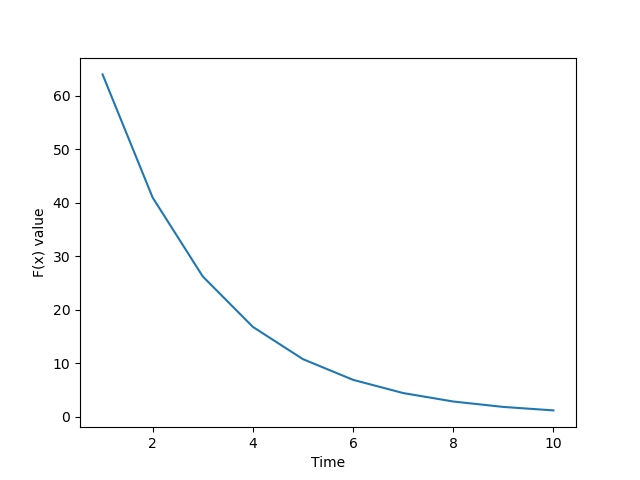
\includegraphics[width=0.7\linewidth]{images/Lab1/LR01.png}
            \caption{F(x) value for 0.1 learning rate}
        \end{figure}
    \newpage
    \item For \(lr=0.01\)
        \begin{figure}[h!]
            \centering
            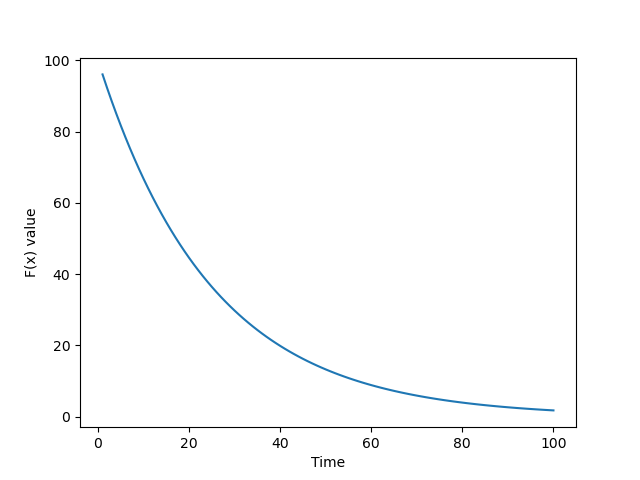
\includegraphics[width=0.7\linewidth]{images/Lab1/LR001.png}
            \caption{F(x) value for 0.01 learning rate}
        \end{figure}

    \item For \(lr = 1.1\)
        \begin{figure}[h!]
            \centering
            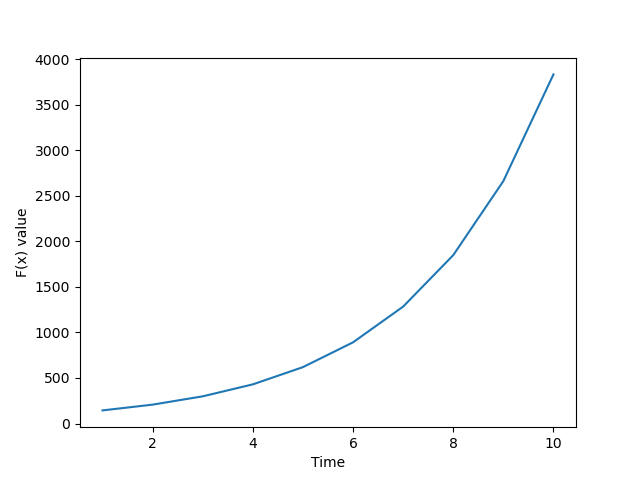
\includegraphics[width=0.7\linewidth]{images/Lab1/LR11.png}
            \caption{F(x) value for 1.1 learning rate}
        \end{figure}
\end{itemize}

By change learning rate to \(0.01\) and \(1.1\), I can conclude that learning rate too low will cause the function take a lot of time to converge and learning rate too high would make it diverge.

\end{document}







